\documentclass[12pt, a4paper]{report}
\usepackage[top=1.0in, bottom=1.0in, left=0.8in, right=0.8in]{geometry}

\setlength{\parskip}{\baselineskip}%
\setlength{\parindent}{0pt}%
\usepackage[]{graphicx}
\usepackage{enumitem}
\usepackage{amsmath}
\usepackage{relsize}
\usepackage{cprotect}
\usepackage{amsmath, amsfonts}
\usepackage{siunitx}
\usepackage{mathrsfs}
\usepackage{framed}
\usepackage{enumitem}
\usepackage{tikz}
\usepackage{circuitikz}
\usepackage{float}
\usepackage[english]{babel}
\usepackage{blindtext}

\hyphenpenalty=10000

\newlist{notes}{enumerate}{1}
\setlist[notes]{label=\textbf{Note:} ,leftmargin=*}

\newlist{hints}{enumerate}{1}
\setlist[hints]{label=\textbf{Hint:} ,leftmargin=*}

\usepackage{xcolor}
\usepackage{color}
\definecolor{com1}{RGB}{125,125,125}
\definecolor{comment}{RGB}{140,115,115}
\definecolor{numbering}{rgb}{0.2,0.2,0.2}
\definecolor{key}{RGB}{0,0,180}
\definecolor{in}{RGB}{0,100,0}
\definecolor{out}{RGB}{100,30,30}
\definecolor{bg}{RGB}{245,245,245}
\definecolor{bgLight}{RGB}{250,250,250}
\definecolor{string}{RGB}{0,150,0}

\usepackage{hyperref}
\hypersetup{
    colorlinks=true,
    linkcolor=blue,
    filecolor=magenta,      
    urlcolor=blue,
}
\urlstyle{same}

\usepackage{listings}

\lstdefinestyle{py_code}{ %
    backgroundcolor=\color{bg},      % choose the background
    basicstyle=\ttfamily\small,		      % fonts
    breakatwhitespace=false,         % automatic breaks at whitespace ?
    breaklines=true,                 % sets automatic line breaking
    captionpos=b,                    % caption-position - bottom
    commentstyle=\itshape\color{comment},    % comment style
    extendedchars=true,              % use non-ASCII
    frame=single,	                   % single frame around the code
    keepspaces=true,                 % keeps spaces in text
    keywordstyle=\bfseries\color{key},% keyword style
    language=Python,                 	  % the language of the code
    morekeywords={Null},       % add more keywords to the set
    numbers=left,                    % line_numbers (none, left, right)
    numbersep=10pt,                  % line_no - code dist
    numberstyle=\footnotesize\color{numbering}, % line_no style
    rulecolor=\color{black},         % frame_color [!always set]
    showspaces=false,                % show spaces everywhere
    showstringspaces=false,          % 
    showtabs=false,                  % 
    stepnumber=1,                    % step b/w two line-no
    stringstyle=\color{string},     % string literal style
    tabsize=2,	                       % sets default tabsize to 2 spaces
    title=\lstname,                  % show the filename
    escapeinside={(*}{*)},			  % escape from style inside (* *)
    xleftmargin=\parindent,
    belowskip=-1.3 \baselineskip,
    aboveskip=1.0 \baselineskip,
    columns=fullflexible,
    xleftmargin=0.15in,
}
\lstnewenvironment{py_code}
{\lstset{style=py_code}}
{}

\lstdefinestyle{psudo}{ %
    backgroundcolor=\color{bgLight},   % choose the background
    basicstyle=\ttfamily\small,		      % fonts
    breakatwhitespace=false,         % automatic breaks at whitespace ?
    breaklines=true,                 % sets automatic line breaking
    captionpos=b,                    % caption-position - bottom
    commentstyle=\itshape\color{com1},          % comment style
    extendedchars=true,              % use non-ASCII
    keepspaces=true,                 % keeps spaces in text
    language=C,                 	  % the language of the code
    morekeywords={type,NULL, True, False},       % add more keywords to the set
    showspaces=false,                % show spaces everywhere
    showstringspaces=false,          % 
    showtabs=false,                  % 
    tabsize=2,	                       % sets default tabsize to 2 spaces
    title=\lstname,                  % show the filename
    escapeinside={(*}{*)},			  % escape from style inside (* *)
    belowskip=-1.8 \baselineskip,
    aboveskip=0.9 \baselineskip,
    columns=fullflexible,
    xleftmargin=0.2in,
    frame=tb,
    framexleftmargin=16pt,
    framextopmargin=6pt,
    framexbottommargin=6pt, 
    framerule=0pt,
}

\lstnewenvironment{psudo}
{\lstset{style=psudo}}
{}

\graphicspath{ ./ }


\title{\textbf{EE2703 : Applied Programming Lab \\ Assignment 3 \\ Fitting Data to Models}} 
\author{V. Ruban Vishnu Pandian \\ EE19B138} % Author name

\date{\today} % Date for the report

\begin{document}		
		
\maketitle % Insert the title, author and date

\section*{Aim}
The aim of this assignment is to:
\begin{itemize}
  	\item Record data from a noisy environment
  	\item Fit the data using a given model
	\item Observe how the fitting model parameters are affected by the noise
 \end{itemize}

\section*{Procedure}
Run the python file ``generate\_data.py'' to generate a set of data following the equation:
 
 \begin{equation}\label{eq:1}
f(t)=1.05J_{2}(t)-0.105t+n(t)
 \end{equation}
 With n(t) being the noise. The noise in each data set follows the normal disribution,
 \begin{equation*}
\mathrm{P}(n(t)|\sigma)=\frac{1}{\sigma\sqrt{2\pi}}\text{exp}\left(-\frac{n(t)^{2}}{2\sigma^{2}}\right)
 \end{equation*}
 
 where $\sigma$ is generated using python function ``logspace''

\begin{psudo}
sigma=logspace(-1,-3,9)
\end{psudo}

The model function which is used to fit the data is,
\begin{equation}\label{eq:2}
g(t;A,B)=AJ_{2}(t)+Bt
\end{equation}
with true values of A and B being
\begin{equation*}
A=1.05,\ B=-0.105
\end{equation*}

The different values of $t$ are known. Also, $t$ is treated as a column vector with different values of time. With this understanding, matrices named $M$ and $p$ are created, where $M$ is a 2-column matrix with the following columns:

First column: Contains the Bessel function $J_{2}(t)$ values for different values of $t$\\
Second column: Is the $t$ vector itself

$p$ matrix is a single 2 element column vector where the first element is $A$ and second element is $B$

We have:
\begin{equation}\label{eq:3}
g(t;A,B)=
\begin{pmatrix}
J_{2}(t_{1}) & t_{1}\\
... & ... \\
J_{2}(t_{m}) & t_{m}
\end{pmatrix}
\cdot
\begin{pmatrix}
A\\B
\end{pmatrix}
=M\cdot p
\end{equation}

Now the mean squared error of the data is found for $A = 0,0.1,...,2$ and $B = -0.2,-0.19,...0$ using the formula
\begin{equation}\label{eq:4}
\epsilon_{ij}=\frac{1}{101}\sum_{k=0}^{101}\left(f_{k}-g(t;A,B)\right)^{2}
\end{equation} 
 
A contour plot of the mean squared error with the values of $A$ and $B$ gives an estimate on the values of A and B where the error reaches its minimum

An estimate of the values of $A$ and $B$ to fit the given noisy data is found using the method of least squares. The required python command is:

\begin{psudo}
scipy.linalg.lstsq(M,Data_to_be_fitted)
\end{psudo}

This gives an estimate for $A$ and $B$ which minimizes the mean squared error.

\subsection*{Results and plots}
\begin{enumerate}
\item The plots of the different noisy datasets to be fitted:
\begin{figure}[H]
    \centering
	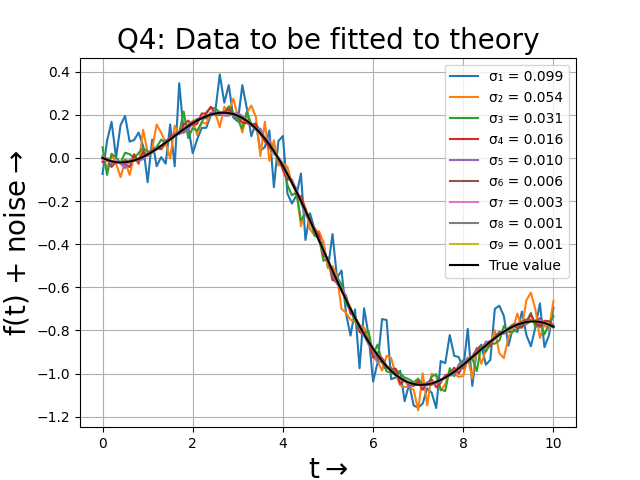
\includegraphics[scale=0.84]{Figure_0} 
	\caption{Data Plot}
	\label{fig:rawdata}
\end{figure}
\clearpage

\item Errorbars are used to show the deviation of the noisy data (with standard deviation 0.1) from the true value:
\begin{figure}[H]
    \centering
	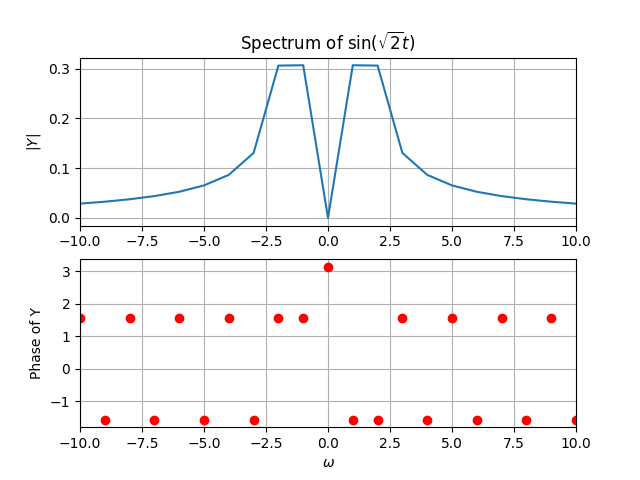
\includegraphics[scale=0.75]{Figure_1}
	\caption{Error Bars}
	\label{fig:errobars}
\end{figure}

\item Contour plot of the mean squared error with various combinations of $A$ and $B$:
\begin{figure}[H]
    \centering
	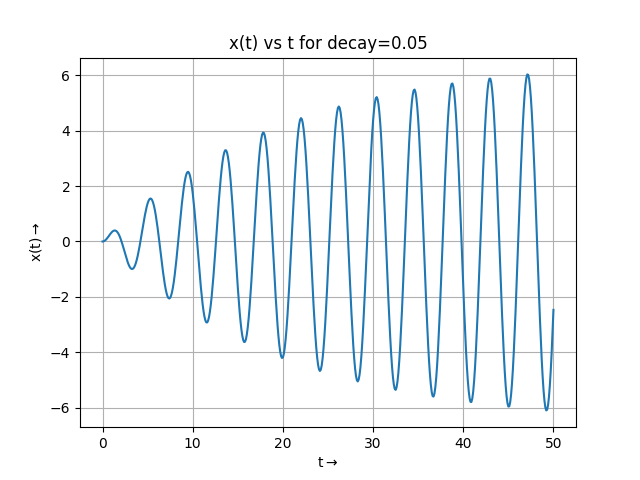
\includegraphics[scale=0.8]{Figure_2}
	\caption{Contour Plot}
	\label{fig:contour}
\end{figure}

\clearpage
\item The plot of deviation of parameters $A$, $B$ from the true values with respect to the standard deviation of the noise present in the data (Linear scale) :
\begin{figure}[H]
    \centering
	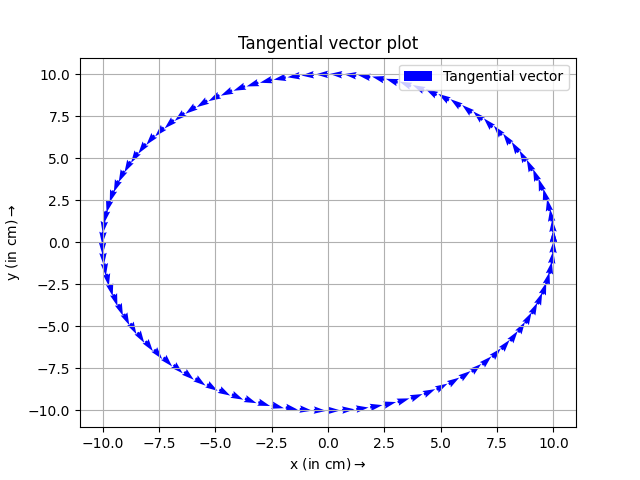
\includegraphics[scale=0.65]{Figure_3}
	\caption{Linear scale error plot}
	\label{fig:eplot}
\end{figure}
The deviation of $A$ is more susceptible to noise more than the deviation of $B$. 

\item The plot of deviation of parameters $A$, $B$ from the true values with respect to the standard deviation of the noise present in the data (Logarithmic scale):
\begin{figure}[H]
    \centering
	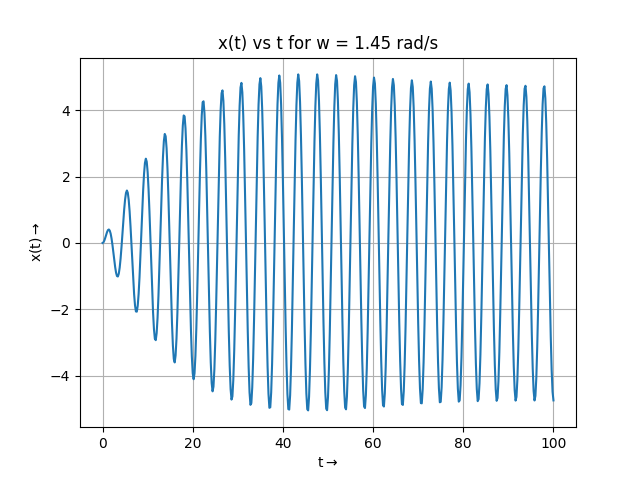
\includegraphics[scale=0.65]{Figure_4}
	\caption{Logarithmic scale error plot}
	\label{fig:logplota}
\end{figure}
The logarithmic errors of $A$, $B$ show somewhat linear behaviour with few deviations from the linear fashion
\end{enumerate}

\subsection*{Observations and Conclusions}
My conclusions are:

\begin{enumerate}
    \item From the contour plot, it is observed that the mean squared error converges to a 
    minimum value as $A$ and $B$ approach their true values which are 1.05 and -0.105. And
    also, there are no multiple minima. There's only a single minimum and that is the least square solution of $A$, $B$. 
    \item The errors in estimate of $A$, $B$ are not varying in a linear fashion with respect to the noise. Also, error in $A$ is more susceptible to noise, implying the Bessel's function values provide more contribution in compensating the noise than the time values do. 
    \item Logarithmic errors of $A$ and $B$ are linearly varying with respect to the logarithm of noise with some deviations. This linear variation means that the errors in estimate of $A$, $B$ are exponents of standard deviation of the noise which is also evident from Figure 4.
    
    \\(Let $\epsilon_{A}$ = Error in A, $\sigma$ = Standard deviation. Then we have:
    log($\epsilon_{A}$) = $k$$\cdot$log($\sigma$)+$c$. 
    \\Hence, $\epsilon_{A}$ = $e^{c}\cdot{\sigma^k}$, where $k$ and $c$ are coefficients
    in the linear relation. Similar relation follows for $\epsilon_{B}$ (Error in B))
\end{enumerate}
\end{document}

